\section{Introduction}
\label{sec:intro}
\subsection{Motivation}
The problem of recovering a signal (or image) from its nonlinear observations is widely encountered in the domain of signal processing, signal acquisition and imaging systems. One such example is the classical problem of phase retrieval, which arises in numerous imaging applications including ptychography, diffraction imaging and astronomical imaging. In such imaging systems, due to the limitations of the optical sensors, only the magnitude of the light rays can be measured but not the phase. As each linear observation losses its phase, the effective forward model can be expressed as a composition of nonlinear absolute value function with the linear observation function. Though the phase retrieval problem is challenging ill-posed inverse problem, it is well-studied in the literature and there exists multiple provably efficient algorithmic procedures to solve it in different settings. \cite{}\todo{cite}

Most of the image and signal acquisition systems suffer from the problem of limited dynamic range. It is well known that real signals contain a large range of intensity levels, and not all of them can be accurately captured due to hardware limited dynamic range of conventional acquisition systems. If tuned incorrectly, most intensity levels can lie in the saturation region of the sensors, causing loss of information through clipping of signals. The problem gets amplified in the case of multiplexed imaging systems, where required dynamic range is very high because of the fact that the observed signal intensity is a sum of various weighted versions of the original signal. The obvious solution to this issue is to increase the dynamic range of the sensors, but unfortunately it is not always possible due to expensive hardware. An alternative approach is the deploy a specifically designed sensors named modulo sensors. As the name suggests, such sensor wraps the observed signal intensity value over given dynamic range, which is analogous to familiar modulo operation with respect to parameter $R$. Usage of the modulo sensor to capture the linear measurements adds an additional effect of modulo operation over each observation, making the forward model highly nonlinear. Recovery of the underlying signal from such modulo measurements turns out to be a challenging and significant yet rarely studied problem in the domain of signal and image processing. 

For most of the nonlinear inverse problems that were solved in the literature, such results require overcomplete obervations, meaning the number of minimum measurements $m$ require for the signal recovery is higher than the ambient dimension $n$ of the signal itself. For the cases where $m$ and $n$ are large, this requirement puts limitation on computation and storage of the measurements. Thus, in this paper, we focus on solving the problem of modulo recovery with very few number of samples. This can be achieved by assuming that the underlying signal obeys a certain low-dimensional structure. Typically, sparsity in some known basis is used as a structural assumption in many imaging applications as many real signals are known to be sparse in some basis. 

\todo{some drawbacks of the prior work, advantages of our work over others}
\subsection{Setup}
\label{subsec:setup}
We formalize the above discussion as follows. Assume $\mathcal{X} \subseteq \R^n$ to be a given (known) subset in the data space, and consider a signal (or image) $\mb{x}^* \in \mathcal{X}$. We construct $\mathbf{A} = \left[\mathbf{a_1~a_2~...~a_m}\right]^T$ with i.i.d. Gaussian entries. We aim to recover the original signal $\mb{x^*}\in \R^n$ from its compressed modulo measurements $y_i$ defined as:
\begin{equation}
y_i=\mod(\langle \mathbf{a_i} \cdot \mathbf{x^*} \rangle,R)~\textnormal{for}~i = \{1,2,...,m\},
\label{eq:modmeas1}
\end{equation} 
where $\mod(\cdot)$ is modulo operation with respect to a fixed, real-valued parameter $R$. We set $m<n$. For simplicity, we assume that the modulo function operates only within two periods, one each on the either side of the origin, as shown in the Fig.~\ref{fig:modop}. The primary assumption in our model is that the natural signal $\mathbf{x^*}$ is $s-$sparse in a chosen basis. 

\begin{figure}[h]
	\begin{center}
		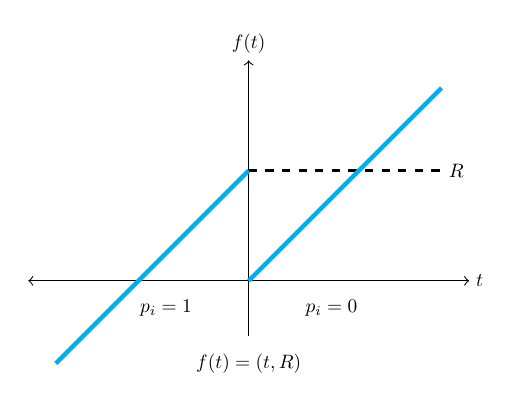
\begin{tikzpicture}[scale=0.7, every node/.style={scale=0.7}]
		\draw[<->] (-4,0) -- (4,0) node[right] {$t$};
		\draw[->] (0,-1) -- (0,4) node[above] {$f(t)$};
		\draw[scale=0.5, dashed, thick] (0,4)--(7,4) node[right]{$R$};
		\draw (1.5,-0.5) node(below) {$p_i = 0$};
		\draw (-1.5,-0.5) node(below) {$p_i = 1$};
		\draw (0,-1.5) node(right) {$f(t) = \mod(t,R)$};
		\draw[scale=0.5,domain=-7:0,smooth,variable=\x,cyan, ultra thick] plot ({\x},{\x+4});
		\draw[scale=0.5,domain=0:7,smooth,variable=\x,cyan, ultra thick]  plot ({\x},{\x});
		\end{tikzpicture}
	\end{center}
	\caption{\emph{Modified modulo function for the given problem}}
	\label{fig:modop}
\end{figure}

\subsection{Our contributions}
\subsection{Techniques}
The proposed MoRAM algorithm is conceptually simple yet novel step in the direction of solving the problem of modulo recovery. Our work takes a fresh approach for solving the modulo recovery problem by borrowing the ideas from the well studied field of phase retrieval and compressive sensing - which has been done for the first time to the best of our knowledge.



\subsection{Paper organization}
The reminder of the paper is organized as follows. In section~\ref{sec:prior}, we briefly discuss the prior work. Sections~\ref{sec:prelim} contains notation and mathematical model used for our analysis. In section~\ref{sec:algo}, we introduce the MoRAM algorithm, and provide a theoretical analysis of its performance. We demonstrate the performance of our algorithm by providing series of numerical experiments in section~\ref{sec:exp}. Section~\ref{sec:disc} provides concluding remarks.